\documentclass[german]{article}
\usepackage[T1]{fontenc}
\usepackage[german]{babel}
\usepackage{graphicx}
\usepackage{ragged2e}
\usepackage{minted}
\usepackage[none]{hyphenat}
\usepackage{pgfplots}
\usepackage{pgfplotstable}
\pgfplotsset{compat=newest}
\usepackage{geometry}
\geometry{left=2cm, right=3cm, top=3cm, bottom=3cm}
\title{Suche nach dem B-A-C-H Motiv \\in gewählten Werken von J.S. Bach}

\date{6. April 2026\\ 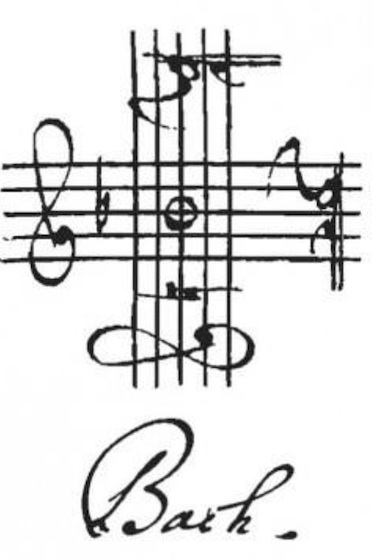
\includegraphics[height=12cm]{BachCrossmoniker.jpg}}
\author{Oskar Nitzschker}

\begin{document}
  
  \justifying
  \pagenumbering{gobble}
  \maketitle
  \newpage
  \pagenumbering{arabic}
  \section{Einleitung}

  Das Konzept der Vertonung des eigenen Namens ist, bzw. war ein beliebtes Konzept unter Komponisten diverser Epochen. Die bekannteste Umsetzung ist das B-A-C-H Motiv von Johann Sebastian Bach. In dem letzten Contrapunktus Satz der Kunst der Fuge erschein das Motiv als Subjekt der dritten Fugenthemas. 
  Im Folgenden werde ich beschreiben wie ich den music21 Bachcorpus und MXL-Dateien nach dem B-A-C-H Motiv durchsucht habe.

  \section{Prozess}
  \subsection{Datenbeziehung}
  Die Untersuchung des music21 Corpus nach allen Werken von J.S. Bach lässt sich in einer Zeile Code programmieren: 
  \begin{minted}{python}
  bachCorpus = m21.corpus.search('bach', 'composer')
  \end{minted}
  Die Variable \mintinline{py}{bachCorpus} enthält eine Liste aller von \mintinline{py}{m21.corpus.search()} gefundener Werke im MXL Format.
  Die Suche nach externen XML-Dateien ist ebenfalls simpel:
  \begin{minted}{python}
  Directory = 'KdF/'
  MXLFiles = []
  for file in os.listdir(Directory):
    if file.endswith('.mxl'):
      MXLFiles.append(file)
  \end{minted}
  Hier wird der Ordner \mintinline{py}{KdF} nach allen Dateien mit der Dateinendung .mxl untersucht. Alle gefunden Ergebnisse werden folgend der Liste \mintinline{py}{MXLFiles} angehängt.
  \subsection{Suchfunktion}
  Sämtliche gesammelten .mxl Dateien werden iterativ der Funktion \mintinline{py}{findMotivFromMXL} übergeben. Diese Funktion beinhaltet zwei Unterfunktionen:
  \begin{itemize}
    \item \mintinline{py}{generateFlatScore()}
    \item \mintinline{py}{findMotiv()}
  \end{itemize}
  Für \mintinline{py}{generateFlatScore()} wird die .mxl Datei erst über die music21 Funktion \mintinline{py}{coverter.parse()} zu einem von music21 verstehbaren Format konvertiert. \mintinline{py}{generateFlatScore()} gibt innerhalb einer Liste seperat alle Stimmen aus. Die einzelnen Stimmen bestehen nur aus Noten und Pausen. Dementsprechend ist das ausgegebene Listenformat: \newline [[Noten \& Pausen aus Stimme 1], [Noten \& Pausen aus Stimme 2], [usw.]]
  Die zweite Funktion \mintinline{py}{findMotiv()} benötigt zwei Eingaben: 1. Die Noten \& Stimmen Liste aus der vorherigen Funktion und 2. Das gesuchte Motiv. Dort anzumerken ist, dass das Motiv vorher in eine Intervalliste umgewandelt wurde, dazu im nächsten Unterabschnitt mehr. Die Funktion sieht folgend aus:
  \begin{minted}{python}
  def findMotiv(flatScore, motiv):
  AmountOfParts = len(flatScore)
  lenMotiv = len(motiv[0])
  foundMotives = [[],[]]
  for i in range(AmountOfParts):
    lenPart = len(flatScore[i])
    for j in range(lenPart):
      currentInterval = convertToIntervals(flatScore[i][j:j+lenMotiv])  
      if currentInterval == motiv[0]:
        foundMotives[0].append((i,(flatScore[i][j][1]+1)))
      elif currentInterval == motiv[1]:
        foundMotives[1].append((i,(flatScore[i][j][1]+1)))
      else:
        pass
  return (len(foundMotives[0]), len(foundMotives[1])) 
  \end{minted}
  Die Funktion schaut sich ein Abschnitt (in der Länge des gesuchten Motivs) innerhalb einer Stimme an, vergleicht diesen mit dem Motiv und speichert den Index des Starttons, falls der Abschnitt mit dem Motiv übereinstimmt. 
  \subsection{Motive \& Intervalle}
  Um die Suche nach Transpositionen einfacher zu gestalten, benötigt \mintinline{python}{findMotiv()} das Motiv in der Form von Intervallen. Die Umrechnung in Intervallen findet für das Motiv in der Funktion \mintinline{py}|generateMotiveIntervals()| statt, während die untersuchten Abschnitte in der Funktion \mintinline{py}|convertToIntervals()| konvertiert werden. Beide Funktionen berechnen die Intervalle durch die Subtraktion der entsprechenden MIDI-Werte.
  \subsubsection{Anmerkung zu den Motiven}
  Mit einem Blick fällt auf, dass das gesuchte Motiv nur zwei Variationen enthält. Zufälligerweise sind die Intervalle der Original Motiv und der Krebs-Umkehrung, sowie der Umkehrung und der Krebsform die Gleichen. Demnach reduziert sich die zu suchende Anzahl von vier auf zwei. 
  \section{Datenauswertung}
  Wie Anfangs beschrieben, werden sämtliche MXL-Dateien iterativ untersucht. Die Ergebnisse werden in einer Liste der Form [Name, Anzahl Original, Anzahl Krebsform] (und ihre Äquivalente) gespeichert. Mit Hilfe der Python Module \mintinline{py}|Pandas| und \mintinline{py}|MatPlotLib| werden diese Ergebnisse in einer .csv Datei gespeichert und abschließend dargestellt.
  \begin{center}
    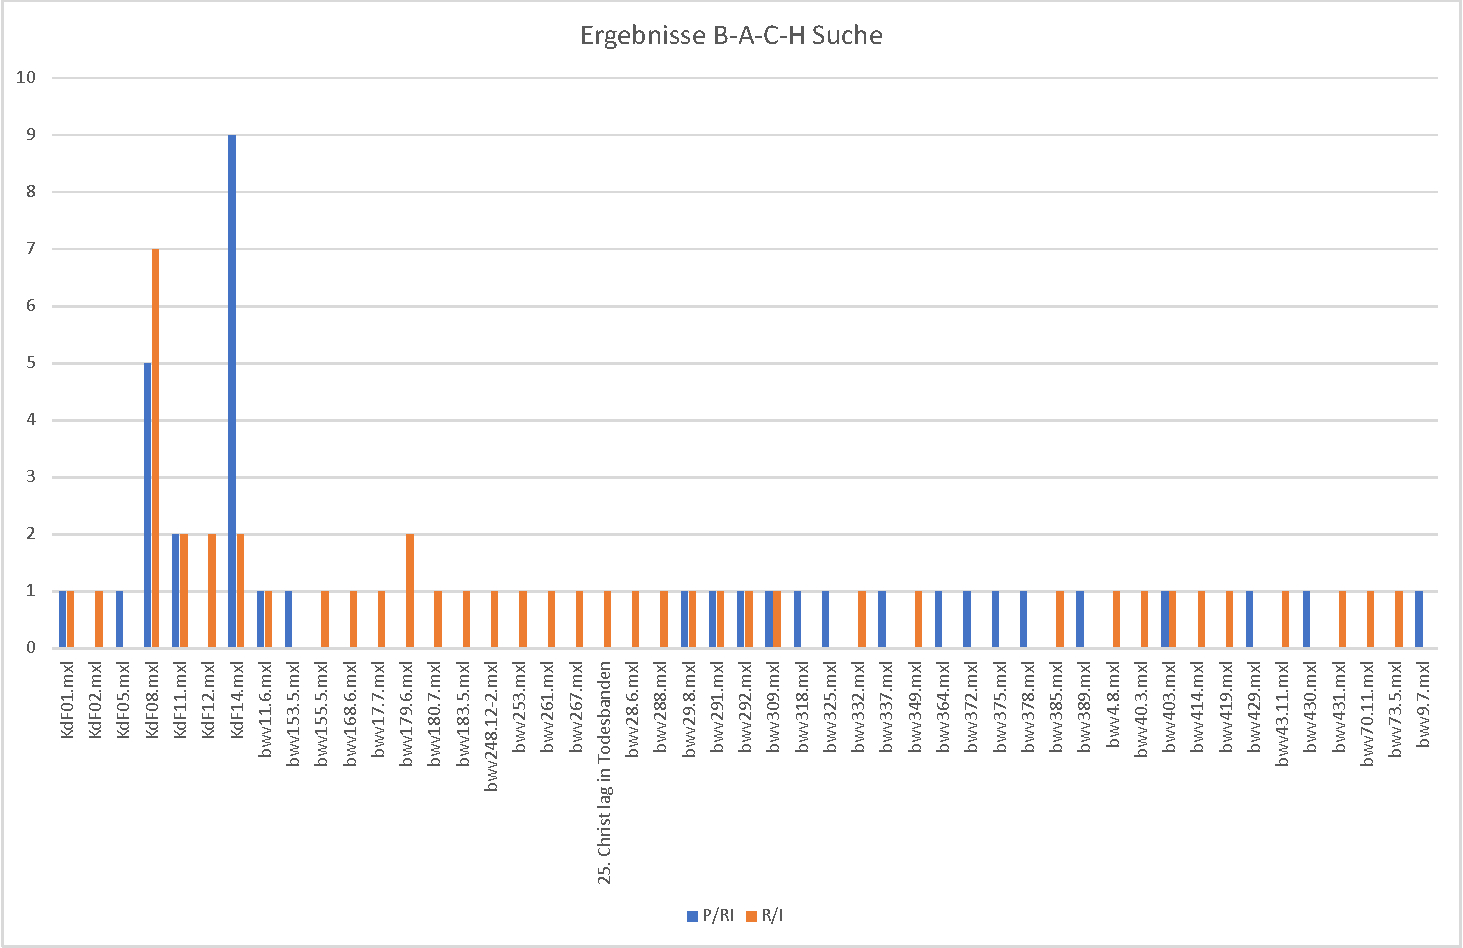
\includegraphics[scale=0.5]{ExcelPDF.pdf}
  \end{center}
\end{document}